\subsection{Design}
Server struktur ses i UML diagram på figur~\ref{fig:ConnectionServer}
\begin{figure}
\centering
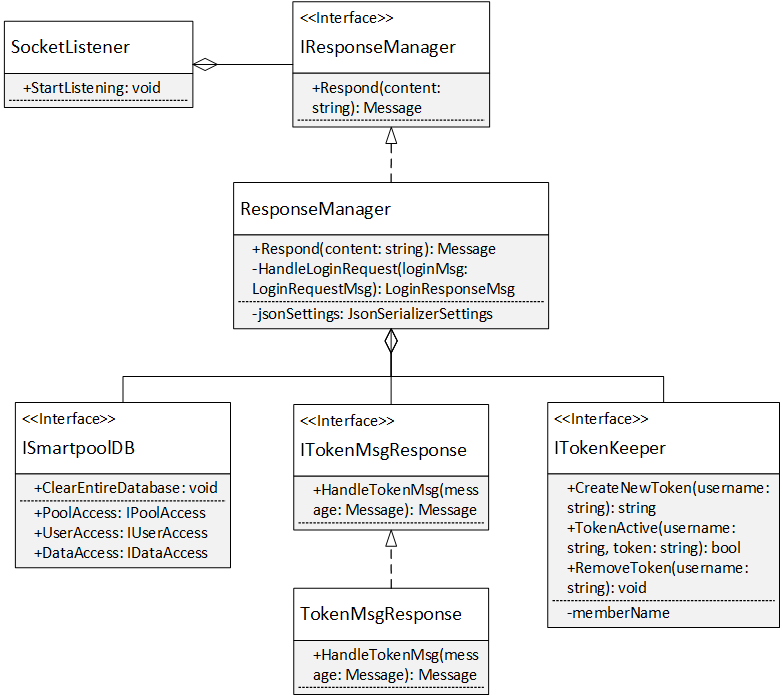
\includegraphics[width=0.9\linewidth]{figs/connection/ConnectionServer.png}
\caption{Server diagram}
\label{fig:ConnectionServer}
\end{figure}

Et typisk forløb i serveren er vist på figur~\ref{fig:ServerSequenceResponse}
\begin{figure}
\centering
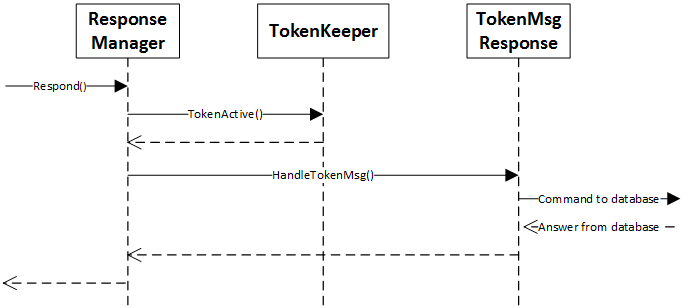
\includegraphics[width=0.9\linewidth]{figs/connection/ServerSequenceResponse.png}
\caption{Server Sequence Diagram}
\label{fig:ServerSequenceResponse}
\end{figure}

For at lave et user session koncept, er der implementeret et token system, som består af en TokenKeeper, Token og TokenStringGenerator klasse. UML diagram over disse ses på figur~\ref{fig:ConnectionServerToken}
\begin{figure}
\centering
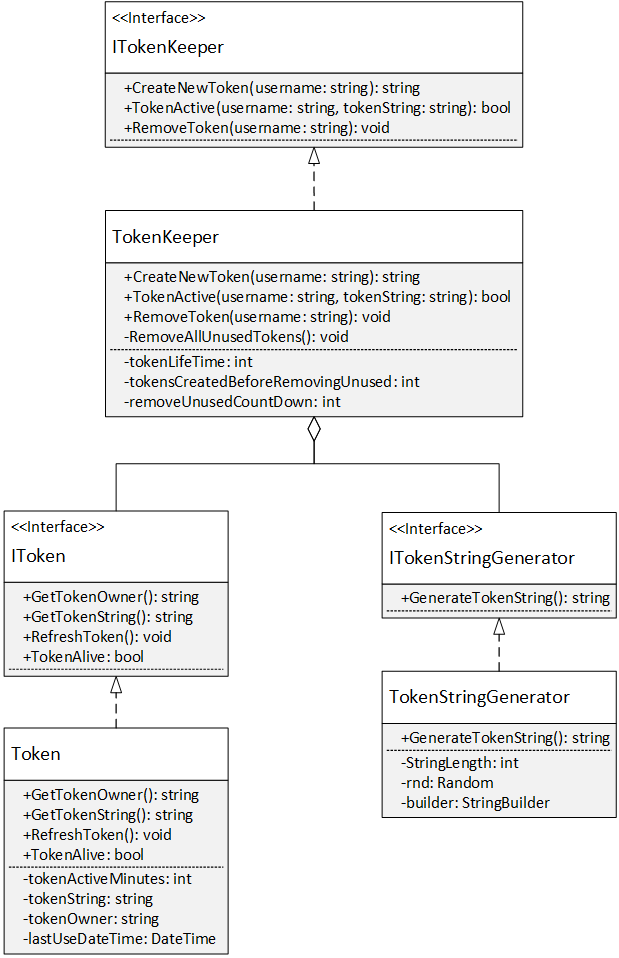
\includegraphics[width=0.7\linewidth]{figs/connection/ConnectionServerToken.png}
\caption{Connection.Server.Token}
\label{fig:ConnectionServerToken}
\end{figure}

For at simulere data fra pools i systemet, er der implementeret en række pool/sensor klasser. Disse ses på figur~\ref{fig:ConnectionPool}
\begin{figure}
\centering
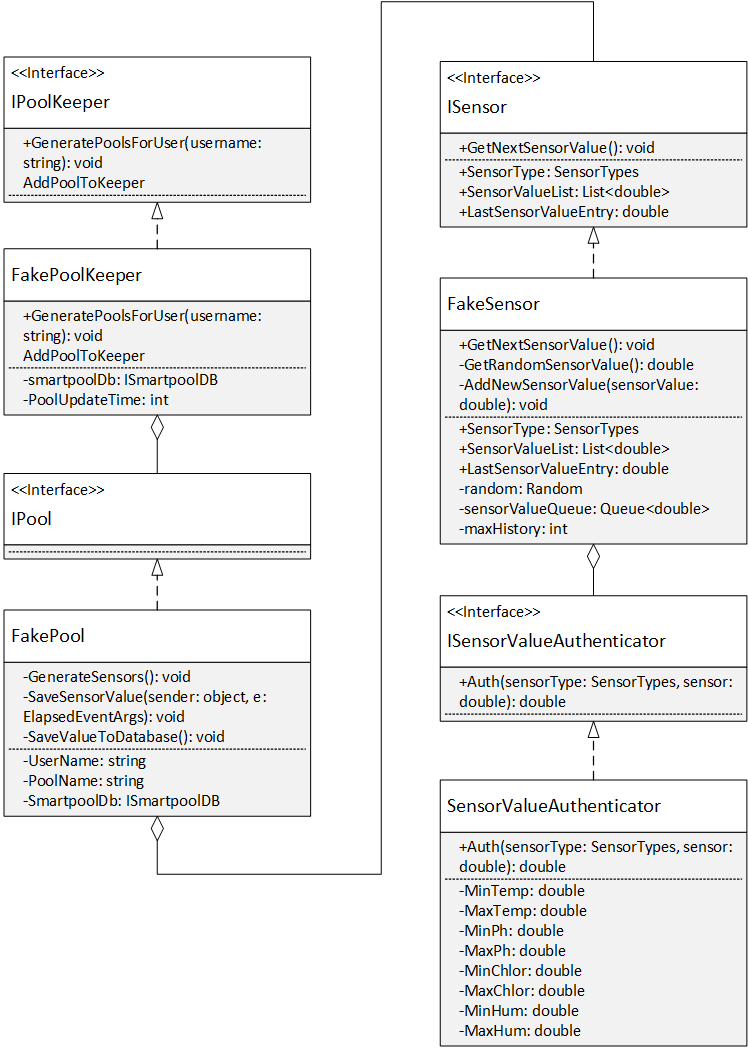
\includegraphics[width=0.8\linewidth]{figs/connection/ConnectionPool.png}
\caption{Connection.Pool diagram}
\label{fig:ConnectionPool}
\end{figure}

\subsection{Implementering}
I denne sektion er beskrevet hvorledes serveren er opbygget. Serveren står for at modtage strings, omdanne dem til besked objekter og lave tilsvarende kald til databasen efter behov. Desuden simuleres pool data i serveren, og der holdes styr på user sessions vha. en TokenKeeper. 

\subsubsection{Asynchronous Socket Listener}
Den primære funktionalitet af denne klasse er hentet fra https://msdn.microsoft.com/en-us/library/fx6588te(v=vs.110).aspx ?? . Denne fungerer ved at køre asynchront, hvilket vil sige at applikationen ikke idler når der afventes en connection. Dette vil med andre ord sige, at der kan oprettes flere forbindelser til serveren på samme tid, da de ikke blokkerer hinanden.
Der er ændret i klassens konsol output, så essentielle data vises. Dette kan ses på figur~\ref{fig:asynchronousSocketListener}

\begin{figure}
\centering
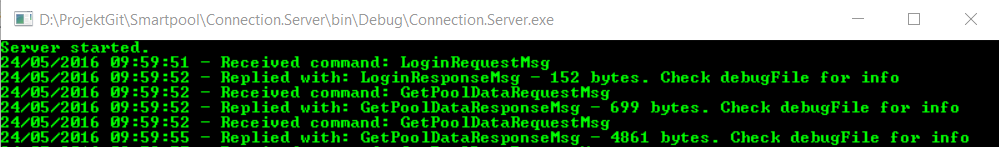
\includegraphics[width=0.9\linewidth]{figs/connection/asynchronousSocketListener.png}
\caption{Asynchronous Socket Listener}
\label{fig:asynchronousSocketListener}
\end{figure}
	
Udfra de viste informationer kan man hurtigt se hvilken type besked der er modtaget, samt hvilken type besked der er svaret med, samt hvor meget denne besked fylder. Det fulde output bliver desuden gemt i en log fil, så det efterfølgende er muligt at se præcis hvilke informationer der er sendt. Dette er valgt for at gøre server vinduet overskueligt, uden at miste essentielle informationer.

Der er desuden valgt at lade exceptions blive vist i server vinduet, som f.eks. ses på figur~\ref{fig:asynchronousSocketListenerException} hvor databasen har genereret en exception, da der er forsøgt at lave et login med et ukendt brugernavn.

\begin{figure}
\centering
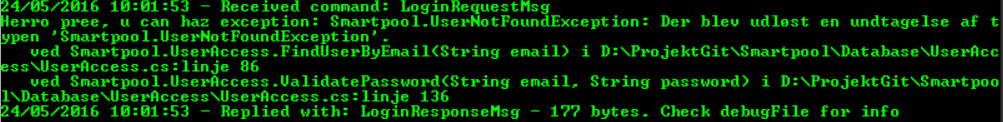
\includegraphics[width=0.9\linewidth]{figs/connection/asynchronousSocketListenerException.png}
\caption{Asynchronous Socket Listener Exception}
\label{fig:asynchronousSocketListenerException}
\end{figure}

Som det også fremgår i server vinduet figur~\ref{fig:asynchronousSocketListenerException} bliver en exception håndteret af serveren, og der sendes en besked af den korrekte type tilbage til klient applikationen, så hverken server eller klient crasher.

\subsubsection{Response Manager}
Denne klasse er primært baseret på en switch case, hvor der baseret på den modtagne beskeds type, returneres et passende svar som set på figur ??
\begin{lstlisting}[caption=Server.ResponseManager, label=code:Server.ResponseManager]
var receivedMessage = JsonConvert.DeserializeObject<Message>(receivedString, _jsonSettings);

switch (receivedMessage.MsgType)
{
	case MessageTypes.LoginRequest:
	var loginMessage = JsonConvert.DeserializeObject<LoginRequestMsg>(receivedString);
	return HandleLoginRequest(loginMessage);
	
	case MessageTypes.TokenMsg:
	var tokenMessage = JsonConvert.DeserializeObject<TokenMsg>(receivedString);
	if (_tokenKeeper.TokenActive(tokenMessage.Username, tokenMessage.TokenString))
	return _tokenMsgResponse.HandleTokenMsg(receivedMessage, receivedString, _tokenKeeper);
	else return new GeneralResponseMsg(false, false);
	
	case MessageTypes.AddUserRequest:
	var addUserMessage = JsonConvert.DeserializeObject<AddUserRequestMsg>(receivedString);
	return new GeneralResponseMsg(false, _smartpoolDb.UserAccess.AddUser(addUserMessage.Fullname, addUserMessage.Username, addUserMessage.Password));

	case MessageTypes.ResetPasswordRequest:
	var resetPasswordMessage = JsonConvert.DeserializeObject<ResetPasswordRequestMsg>(receivedString);
	return new GeneralResponseMsg(false, false);
	
	default:
	return new GeneralResponseMsg(false, false)	{MessageInfo = "The server did not recognize your request"};
}
\end{lstlisting}

Klassens switch-case er indkapslet i en try block, hvori der sørges for at eventuelle exceptions bliver håndteret, og der sendes et passende svar tilbage til klienten. Der er yderligere lavet en metode til håndtering af login requests, da denne som den eneste krævede en længere håndtering. Denne anvender en task til at kalde i databasen, da dette ved test af og til tog længere tid end forventet. Metoden ses på figur ??

\begin{lstlisting}[caption=Server.ResponseManager.HandleLoginRequest, label=code:Server.ResponseManager.HandleLoginRequest]
var task = Task.Run(() => _smartpoolDb.UserAccess.ValidatePassword(loginMsg.Username, loginMsg.Password));
if (task.Wait(TimeSpan.FromSeconds(15))) //if task is completed within time limit
{
	return task.Result ? new LoginResponseMsg(_tokenKeeper.CreateNewToken(loginMsg.Username), true) : new LoginResponseMsg("", false) {MessageInfo = "Username or password was incorrect"};
}
else
	return new LoginResponseMsg("", false) {MessageInfo = "Login timed out. Please try again later"};
\end{lstlisting}

\subsubsection{Token System}
Oprettelse af nye tokens sker ved at kalde metoden CreateNewToken med et username som parameter. Dette username bliver gemt i et token objekt, som også indeholder en token string genereret af TokenStringGenerator, samt en DateTime variabel. DateTime variablen indeholder oplysninger om hvornår denne token sidst blev anvendt/oprettet.
For at undgå at inactive tokens bliver liggende i systemet, sørger TokenKeeper for at tælle en variabel ned, som definerer hvornår den skal rydde op i sin liste af aktive tokens. Til sidst returnerer TokenKeeper den genererede TokenString, som bliver sendt tilbage til klient applikationen. Det hele ses på~\ref{code:ServerTokenKeeperCreateNewToken}
\begin{lstlisting}[caption=Server.TokenKeeper.CreateNewToken, label=code:ServerTokenKeeperCreateNewToken]
public string CreateNewToken(string username)
{
	var newToken = new Token(username, _tokenStringGenerator, _tokenLifeTime);
	_tokens.Add(newToken);
	
	if (_removeUnusedCountdown == 0)
	{
		RemoveAllUnusedTokens();
		_removeUnusedCountdown = _tokensCreatedBeforeRemovingUnused;
	}
	_removeUnusedCountdown--;
	
	return newToken.GetTokenString();
}
\end{lstlisting}

\subsubsection{Pool DataGeneration}
\paragraph{PoolKeeper} er implementeret som en fake klasse, der indeholder en liste over pools i systemet. Ved opstart chekkes på få udvalgte brugernavne i databasen, som der derefter genereres tilsvarende pools for. Desuden bliver der, mens systemet kører, oprettet pools i systemet for nye pools der tilføjes til databasen. Så længe serveren kører, vil alle nye pools altså generere data.

\paragraph{Pool} er implementeret som en fake klasse. Klassen indeholder ikke nogen public metoder, da den er selvkørende og ved et angivet interval selv opretter sensor data i databasen. Dette er tiltænkt at være tilsvarende et reelt system, hvor en reel pool klasse, ved et givet interval, sender en request til en fysisk enhed om måledata, som derefter gemmes i databasen.

Oprettelse af en pool via klassens constructor ses på ??
\begin{lstlisting}[caption=Server.FakePool.Constructor, label=code:ServerFakePoolConstructor]
public Pool(int secondsBetweenSensorReadings, string userName, string poolName, ISmartpoolDB smartpoolDb)
{
	UserName = userName;
	PoolName = poolName;
	SmartpoolDb = smartpoolDb;
	_fakeSensors = new List<ISensor>();
	GenerateSensors();
	var timer = new Timer { Interval = 1000 * secondsBetweenSensorReadings };
	timer.Elapsed += SaveSensorValue;
	timer.Start();
}
\end{lstlisting}

\paragraph{Sensor} er implementeret som en fake klasse. Der er lagt stor vægt på at klassen genererer værdier som kunne være reele, da dette er med til at give et helhedsindtryk af det endelige system. 

\paragraph{SensorValueAuthenticator} som et led i at give sensoren realistiske værdier, er denne klasse oprettet for at angive en minimum og maximum værdi, en given sensor type kan have.